\chapter{Teorema de \emph{Noether} I/II}
\label{NoeterIdeII}

	
\begin{tikzpicture}
	\fill [left color=red!50, right color=teal!50] (0,0) rectangle (6.5,.1);
	\fill [left color=teal!50, right color=blue!50] (6.5,0) rectangle (11.5,.1);
	\end{tikzpicture}



\vspace{10mm}
\begin{adjustwidth}{50pt}{50pt}
\begin{ejemplo}
\begin{multicols}{2}

$\,$

\begin{figure}[H]
	\centering
	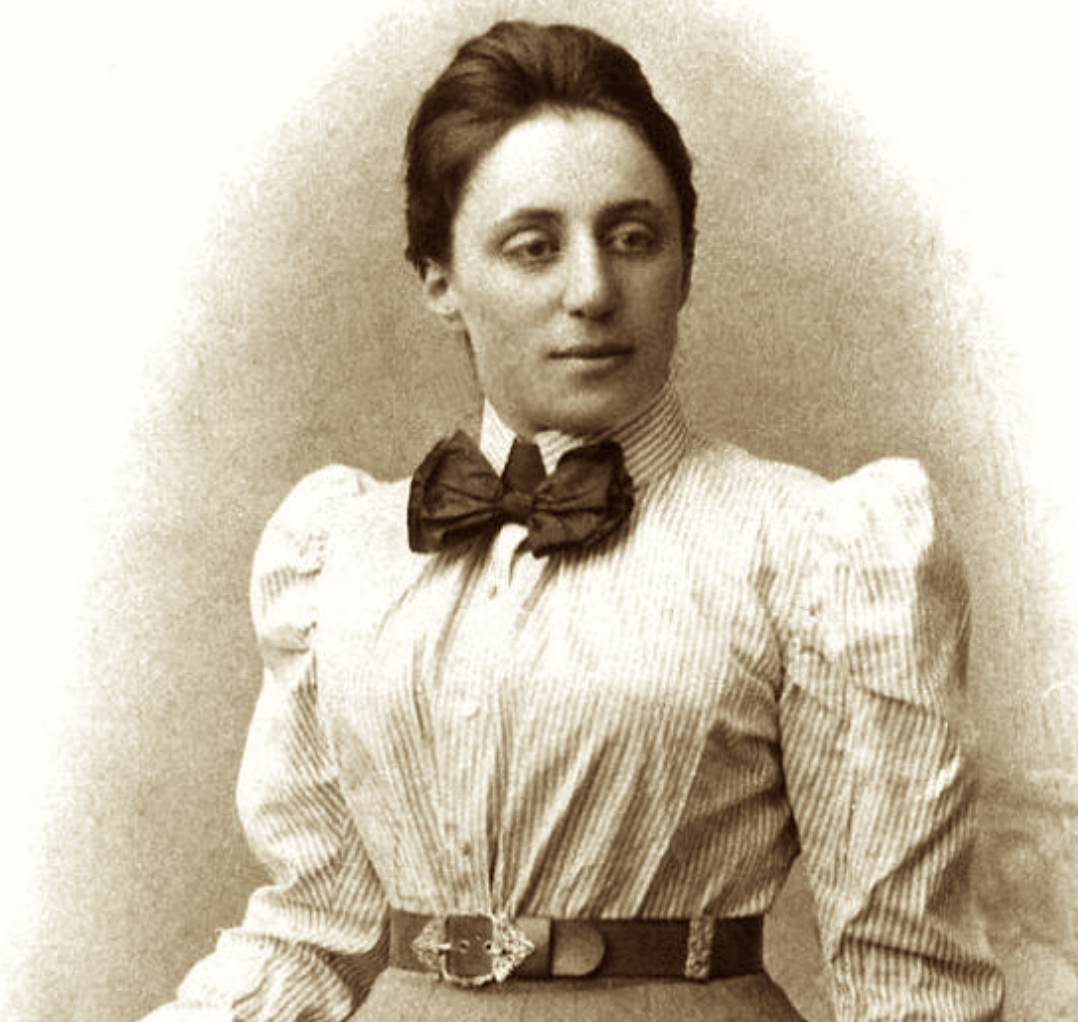
\includegraphics[width=.4\textwidth]{imagenes/img14-01.png}
\end{figure}
Emmy Noether Amalie (Erlangen, Baviera, Alemania, 23 de marzo de 1882 - Bryn Mawr, Pensilvania, Estados Unidos, 14 de abril de 1935) fue una matemática alemana, de ascendencia judía, especialista en la teoría de invariantes y conocida por sus contribuciones de fundamental importancia en los campos de la física teórica y el álgebra abstracta. Considerada por David Hilbert, Albert Einstein y otros personajes como la mujer más importante en la historia de la matemática. En física, el teorema de Noether explica la conexión fundamental entre las simetrías y las leyes de conservación. A pesar de ello, se le negó la posibilidad de un puesto digno en la universidad por el hecho de ser mujer.
\end{multicols}
\end{ejemplo}
\end{adjustwidth}
\vspace{5mm}

\section{Ejemplo introductorio}

\begin{example}
. \begin{multicols}{2}	

	$\,$
	
	\begin{figure}[H]
	\centering
	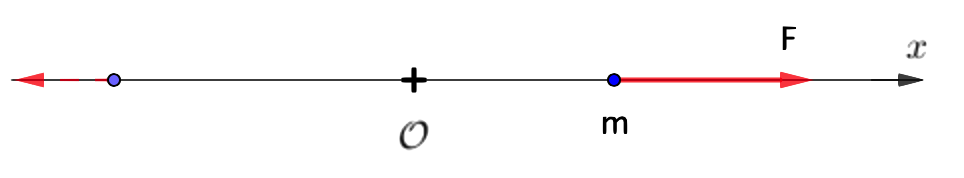
\includegraphics[width=.5\textwidth]{imagenes/img14-02.png}
\end{figure}


$m$ en 1 dimensión sometida a una fuerza $F=2a/x^3$, con la $a$ un valor constante y positivo. 

\vspace{2mm} Tenemos un problema de repulsión desde el origen de coordenadas.
\end{multicols}
\end{example}

Pasos que vamos a realizar:

\vspace{-3mm}  \begin{enumerate}
\vspace{-3mm} \item Construir el lagrangiano.
\vspace{-3mm} \item Buscar que cantidades se conservan.
\vspace{-3mm} \item Buscar si hay algún tipo de simetría que nos lleva a otra cantidad conservada.	
\end{enumerate}

\vspace{-3mm} Con ambas cantidades conservadas podremos obtener la solución del problema sin necesidad de resolver ninguna ecuación diferencial. Estaremos aplicando el teorema de Noether sin saberlo, pero nos servirá de motivación.

\vspace{5mm} ---$\triangleright\ \ 1)\ \ $ $T=\dfrac m 2 \dot x^2;\quad V=-\int F \dd x=-2a\int x^{-3} \dd x=ax_2+C; \ \  V(\infty)=0 \to C=0 \ \ \Rightarrow \ V=\dfrac a {x^2}$

$$\boldsymbol{ L=T-V=\dfrac m 2 \dot x^2 - \dfrac {a}{x^2} }$$

\vspace{5mm} ---$\triangleright\ \ 2)\ \ $ Como $L\neq L(t) \ \to \ H=cte$

$T$ homogénea 2 grado $\ \text{ y } \ $ $V=V(x)$ (solo depende de $x$) $\ \to \ H=E=cte=T+V$

$$\boldsymbol{E=T+V=\dfrac m 2 \dot x^2 + \dfrac {a}{x^2} = cte}$$

La energía se conserva, ya tenemos una de las dos cantidades conservadas que buscamos.

\vspace{5mm} ---$\triangleright\ \ 3)\ \ $ simetría $\ \to \ $ otra cantidad conservada. Vamos a estudiar la \emph{\textbf{acción}}:

$s[x(t)]=\displaystyle \int_{t_1}^{t_2} L(x, \dot x, t) \dd t = \textcolor{gris}{(\ L\neq L(t) \ )} = \int_{t_1}^{t_2} L(x, \dot x) \dd t \, , \ \ $ en nuestro caso,

\begin{equation}
\label{T14accion1}
s[x(t)] \displaystyle  = 
\int_{t_1}^{t_2} \left[ \dfrac m 2 \dot x^2 - \dfrac a{x^2} \right]  \dd t
\end{equation}

Las trayectorias posibles que seguirá la partícula son curvas de la gráfica $x-t$, la trayectoria real será aquella que minimice la acción, $s[x(t)]$ mínima.

Estamos interesados en estudiar la simetría, para ello vamos a inventarnos una curva $x-t$ que no coincidirá con la trayectoria real: nos inventamos, por ejemplo la curva $x(t)=t$ \textcolor{gris}{(partícula moviéndose hacia la derecha a velocidad $v=1=cte$ lo cual es imposible ante la presencia de una fuerza repulsiva que la dota de aceleración, se trata de una trayectoria no real, es inventada)}.


\begin{figure}[H]
	\centering
	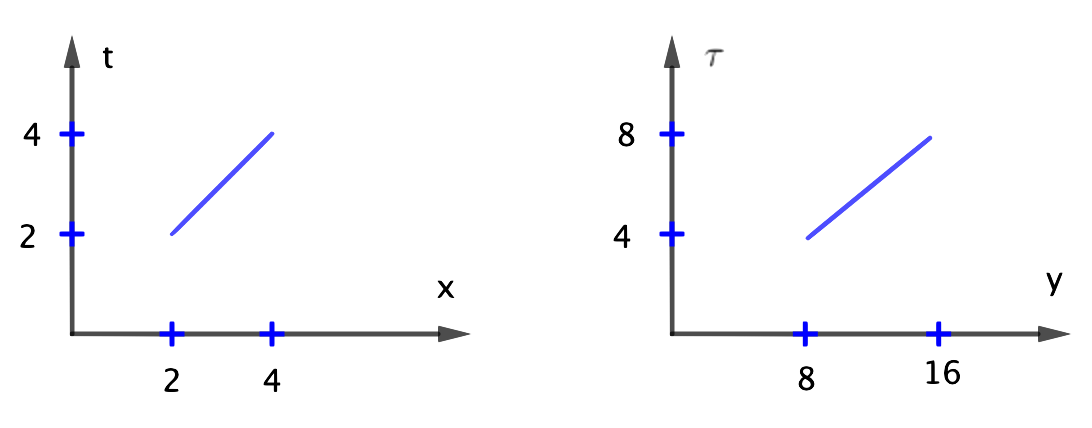
\includegraphics[width=.75\textwidth]{imagenes/img14-03.png}
\end{figure}


Nuestra trayectoria imaginaria es $\ x(t)=t;\ \dot x=1;\ (m=1; \ a=1); \ t\in[2,4]$

$\boldsymbol{ s[x(t)]=}\displaystyle \int_2^4 \left( \dfrac 1 2 \ 1 - \dfrac 1 {x^2} \right) \dd t =   \left[ \dfrac 1 2 \ t + \dfrac 1 t \right]_2^4  \boldsymbol{ =\dfrac 3 4 }$

Inventemos otra curva: $\ y=2x(t)=2t, \ $ con $\ \tau = 4t \to \begin{cases}
 	\ t=2,\ \tau=4,\ \ y=4 \\ \ t=4,\ \tau=16,\ y=8
 \end{cases}$
 
 $\dot y=\dfrac{\Delta y}{\Delta \tau}=\dfrac{8-4}{16-8}=\dfrac 1 2 \quad ; \qquad y(t)=2t;\ \tau=4t \ \to \ y(\tau)=2t(\tau)=2 \left( \dfrac \tau 4 \right) = \dfrac \tau 2$ 

 
Calculemos la acción para esta curva:
$\ \ \boldsymbol{ \displaystyle s[y(t)]}=\int_8^{16} \left[ \dfrac 1 2 \left( \dfrac 1 2 \right)^2 - \dfrac 1 {y^2} \right] \dd \tau=\left[ \dfrac 1 8 \tau + \dfrac 4 \tau \right]=\boldsymbol{ \dfrac 3 4}$
 
\begin{large}
 \begin{center}
 \emph{ ------ $\quad$ !`Da el mismo resultado!} $\quad$ 	------  
 \end{center}
\end{large}
 
Hemos realizado una \emph{transformación}: $\ x,t \ \to \ y,\tau \ $ de modo que la acción no ha variado, es invariante. Esto nos hace pensar que puede existir una simetría, si la ``acción'' es invariante frente a una \emph{familia de transformaciones}.

Pero, si para pasar de $x$ a $y$ hemos multiplicado por $2$, ?`para pasar de $t$ a $\tau$ hay que multiplicar por $4$ o elevar $2$ al cuadrado? Planteemos una transformación similar general y exijamos que la acción quede invariante:

\begin{equation}
\label{T14transf-inv-acc-ejemplo}
y(t) \ = \ \lambda \ x(t) \ , \qquad \tau \ = \ f(\lambda) \cdot t 	 \qquad \to \qquad s[x(t)]\ = \ s[y(\tau)]
\end{equation}

$y(t)=\lambda x(t) \ \to \ \displaystyle \dot y =\dv{y}{\tau}=\dv{y}{x}\dv{x}{\tau}=
\dv{y}{x}\dv{x}{t}\dv{t}{\tau}=\lambda \ \dot x \ \dfrac{1}{f(\lambda)}=\dfrac{\lambda}{f(\lambda)}\ \dot x$

donde hemos usado que $\ \displaystyle \tau=f(\lambda) t \ \to \ \dv{\tau}{t}=f(\lambda) \ \to \ \dfrac{1}{f(\lambda)} = \dv{t}{\tau}$

De aquí,   $\ \displaystyle \dot x= \dfrac{f(\lambda)}{\lambda} \ \dot y =
\dfrac{f(\lambda)}{\lambda} \ \displaystyle \dv{y}{\tau} $

Calculemos la acción $\ \displaystyle s[y(t)]=\int_{t_1}^{t_2} \left[ \dfrac m 2 \left( \dfrac{f(\lambda)}{\lambda} \dv{y}{\tau} \right)^2 - \dfrac {a}{(y/\lambda)^2} \right] \dd t = \int_{\tau_1}^{\tau_2} \left[ \dfrac m 2 \dfrac{f^2}{\lambda^2} \left( \dv{y}{\tau} \right)^2 - \lambda^2 \dfrac{a^2}{y^2} \right] \dfrac{\dd \tau}{f} $

Donde hemos usado, $ \ \tau=f(\lambda) t;\ \quad \lambda \ constante \ \to \ \dd \tau= f(\lambda) \dd t \ \to \ \dd t = \dfrac{\dd \tau}{f}$

 
$\displaystyle  s^y(\tau)] = \int_{\tau_1}^{\tau_2} \left[ \dfrac{f}{\lambda^2} \dfrac m 2 \left( \dv{y}{\tau} \right)^2 -\dfrac{\lambda^2}{f} \dfrac{a}{y^2} \right] \dd \tau$

Procedemos ahora a un cambio de notación, que no de variable (para mejor comparar) : $\ y \leftrightarrow x \ ; \quad t \leftrightarrow \tau$

\begin{equation}
	\label{T14accion2}
	s[x(t)] \ = \ 
	\int_{t_1}^{t_2} \left[ \dfrac{f}{\lambda^2} \dfrac m 2 \left( \dv{x}{t} \right)^2 -\dfrac{\lambda^2}{f} \dfrac{a}{x^2} \right] \dd t
\end{equation}

Para que la acción haya resultado invariante ante esta familia $f(\lambda)$ de transformaciones es necesario que coincidan las ecuaciones \ref{T14accion1} y \ref{T14accion2}:

$$\dfrac f{\lambda^2} = 1 \quad \wedge \quad \dfrac{\lambda^2}{f}=1 \qquad \to \qquad \boxed{\boldsymbol{ \ f \ = \ \lambda^2 \ }} $$

\textcolor{gris}{(La relación antes buscada era elevar al cuadrado y no multiplicar por dos.)}

Acabamos de descubrir una nueva \emph{simetría continua} \textcolor{gris}{(para pasar de unas coordenadas a otras usamos un parámetro real $\lambda$ que puede tomar cualquier valor)} : \ $\subrayado{\quad \boxed{ \ y(t) \ = \ \lambda \ x(t) \, ; \qquad \tau \ = \ \lambda^2 \ t}}$

Veremos que la existencia de una simetría continua asegura la existencia de una nueva cantidad conservada.

La acción tiene una simetría continua que la deja invariante. \textcolor{gris}{Es un caso particular de lo que se llama ``simetría conforme'' (leyes invariantes de escala), se verá más adelante.}


\vspace{5mm}
------  Vamos a imaginar una especie de ``movimiento'' dado por la simetría, podemos imaginar que dada una simetría y una posición $x$ en un tiempo $t$, multiplicamos y obtenemos $\lambda x$, $\lambda^2 t$ y observemos cual es la ``trayectoria''.

$\begin{cases}
\ x\ \to \lambda x \\ \ t \ \to \ \lambda^2 t	
\end{cases} \ \ \lambda=1\ \ (t=1,x=2) \ \to \ (\lambda^2, 2\lambda) =(X,Y) \ \to \quad Y=2\sqrt{X} \ \leftrightarrow \ X=\dfrac {Y^2}4 \,\ \ $ parábola.

Veamos los valores de $L$ en estas posiciones, pero, antes un pequeño cambio: nos gustaría que la posición inicial fuese cuando el parámetro valiese cero y tenemos $\lambda=1$, para corregir esto se nos ocurre:

$\lambda=g(\varepsilon) \ / \ \varepsilon=0 \leftrightarrow \lambda=1 \quad \Rightarrow \quad \boldsymbol{\lambda \ = \ e^{\varepsilon} \, , \ \  }$ fácilmente derivable.

\begin{figure}[H]
	\centering
	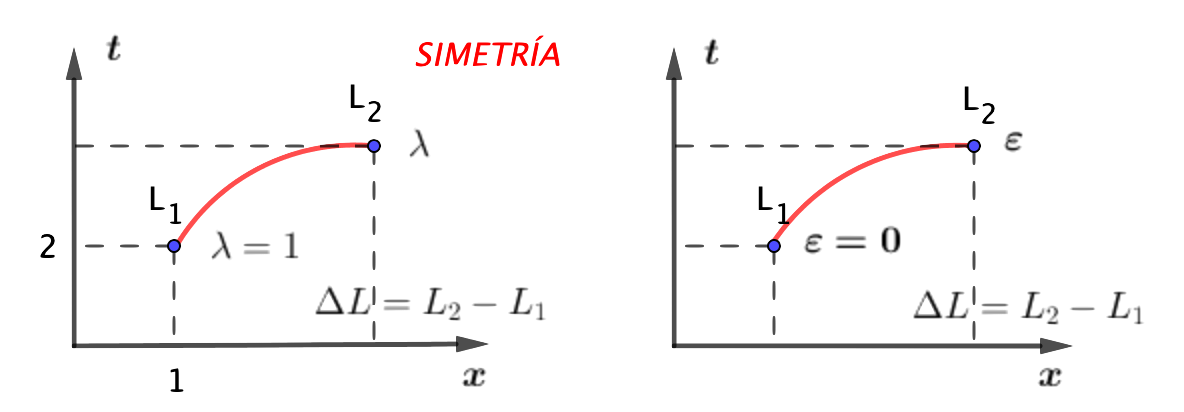
\includegraphics[width=.8\textwidth]{imagenes/img14-04.png}
\end{figure}

Así, tendremos $\quad \ x \ \to \ e^\varepsilon \ ;\qquad t \ \to \ (e^\varepsilon)^2 \ = \ e^{2\varepsilon}$
 
Supongamos que este ``movimiento'' es \emph{infinitesimal}, $\ \varepsilon<<1 \ \to \ \varepsilon^2 \approx 0\, . \ $ Aproximaremos por polinomios de Taylor de primer grado. Calcularemos $\var L$ en lugar de $\Delta L$.

Taylor: $\ \begin{cases} \ y\approx (1+\varepsilon)x(t) \\ \ \tau \approx (1+2\varepsilon)t \end{cases} \qquad \ t=\dfrac {\tau}{1+2\varepsilon} \ \  \to \ \ \  y = (1+\varepsilon) \ x \left( \dfrac{\tau}{1+2\varepsilon} \right) $

Polinomio primer grado Taylor: $\ \ y(\varepsilon) \approx y_0 + y'(0)\cdot \varepsilon$

$\eval{ y'(\varepsilon) }_{\varepsilon=0} \ = \ \eval{ 1 \ x \left( \dfrac{\tau}{1+2\varepsilon} \right) \ + \ (1+\varepsilon) \displaystyle \left( \dv{x}{t} \right) \left( \dfrac{\tau}{1+2\varepsilon} \right) \cdot \tau \dfrac{-1}{(1+2\varepsilon)^2} \cdot 2  \ }_{\varepsilon=0}$

Hemos usado la regla de la cadena: $\quad \displaystyle f\left( g(\varepsilon) \right)' = f' \left( g(\varepsilon) \right) \cdot g'(\varepsilon)\, , \ $ además, $\ \displaystyle \dv{x}{t}=\dot x$ 


$\eval{y'(\varepsilon)}_{\varepsilon=0} \ = \eval{\ x \left( \dfrac{\tau}{1+2\varepsilon} \right) \ - \ (1+\varepsilon)\ \dot x \ \dfrac{2\tau}{(1+2\varepsilon)^2}\ }_{\varepsilon=0} \ = \ x(t) \ - \ 2 \ \dot x(t) \ t$

Sustituyendo el el polinomio de orden 1 de Taylor,

$y(\varepsilon) = y(0)+[x(t)-2\dot x(t) \ t]\cdot \varepsilon\, , \ $ pero $\ y\approx (1+\varepsilon)x(t) \ \to \  y(0)=x(t)\, , \ $ luego

$y(0) \approx x(t) \ + \ [x(t)-2 \dot x \ x(t)]\cdot \varepsilon$


Las ecuaciones de la transformación infinitesimal son


\begin{equation}
\label{T14ecTransInfinitesimal}
\boxed{ \ y \ \approx \ x + (x-2\dot x t)  \  \varepsilon \ }	\ \ ; \qquad \boxed{\    \tau \ \approx \ (1+2\varepsilon)\ t }
\end{equation}


\vspace{5mm} Continuemos nuestro cálculo de la variación de la acción:

$L=\dfrac{m\dot x^2}{2}-\dfrac{a}{x^2} \ \to \ \displaystyle
\var L =\pdv{L}{x}\var x + \pdv{L}{\dot x} \var \dot x = + a \dfrac {2}{x^3} \var x + m\dot x \var \dot x$

$x$ varía desde $x$ hasta $y=x+(x-2\dot x t)\varepsilon \ \to \ \var x = y-x=\varepsilon (x-2\dot x t)$

$t$ varía desde $t$ hasta $\tau=(1+2\varepsilon)t \ \to \ \var  t = \tau - t = 2 \varepsilon t$

Además, $\ \var \dot x = (\var x)' =[\varepsilon(x-2\dot x t) ]'=\varepsilon [\dot x - 2(\ddot x t + \dot x)] =\varepsilon(-\dot x -2\dot x t) \, , \ $ con todo esto,

$\var L = \varepsilon \ \left[ 
\dfrac{2a}{x^2}- \dfrac{4a\dot x t}{x^3} -m\dot x^2 -2m\dot x \ddot x t \right] $

$\var L = 2 \varepsilon \  \left[
\textcolor{red}{\left(  \dfrac{a}{x^2}- \dfrac{m \dot x}{2} \right)} -
\textcolor{blue}{\left( \dfrac{2a\dot x}{x^3} + m\dot x \ddot x \right)} \right] \ t $

Por un lado, $\ \textcolor{red}{\left(  \dfrac{a}{x^2}- \dfrac{m \dot x}{2} \right)} = - L$

Por otro, $\ L=\dfrac{m\dot x^2}{2}-\dfrac{a}{x^2} \ \to \ \displaystyle
\dv{ L}{t} = \dfrac m{\cancel{2}} \cancel{2} \dot x \ddot x - a (-2x^{-3}) \dot x \ \to \  \textcolor{blue}{\left( m\dot x \ddot x +  \dfrac{2a\dot x}{x^3}  \right) = \dv{L}{t} }$

Luego, $\quad \displaystyle \var L \ = \ 2\varepsilon \ \left[ -L - t \cdot \dv{L}{t}\right] \ = \ 2 \varepsilon \ \dv{t} [-t\ L]\ \ \ $  \textcolor{gris}{(derivada del producto).}


\vspace{5mm} 

------ Vamos ahora a plantear un ``movimiento real'', que no tendrá nada que ver con la simetría. Pasamos de un punto en que el lagrangiano vale $L_1$ a otro en que vale $L_2$, si el movimiento es infinitesimal tendremos que la variación es $\ \var L=\displaystyle \pdv{L}{x} \var x + \pdv{L}{\dot x} \var \dot x$

Anteriormente, $\ \var x \text{ y } \var \dot x \ $ venían determinadas por la simetría \textcolor{gris}{($\ \var x=\varepsilon (x-2\dot x t);\ \ \var t=2\varepsilon t \ $)}.

Ahora vamos a imponer que se cumplan las ecuaciones de Euler-Lagrange, que son el sello de garantía de que el movimiento responderá a un caso real: $\ \displaystyle \dv{t} \left( \pdv{L}{\dot x} \right) = \pdv{L}{x}\, , \ $ sustituyendo en $\ \var L\, ,$

$\var L = \displaystyle \dv{t} \left( \pdv{L}{\dot x} \right) \var x + \pdv{L}{\dot x} \var \dot x = \dv{t} \left[  \left( \pdv{L}{\dot x} \right)\cdot \var x \right]\ \ $  \textcolor{gris}{(derivada del producto).}

Tenemos que, $\quad \begin{cases}
 \ \text{Movimiento real} & \displaystyle \var L = \dv{t} \left[  \left( \pdv{L}{\dot x} \right)\cdot \var x \right] \\ \\
 \ \text{Movimiento de la simetría} & \var L = \varepsilon \ [-2tL]
 \end{cases}$

Notación: trayectoria real $x_R(t)$; trayectoria de la simetría $x_S(t)$

Real: $\ \displaystyle \var L(x_R, \dot x_R, \var x) = \dv{t} \left[  \left( \pdv{L}{\dot x} \right)\cdot \var x \right]\, ; \ $ Simetría: $\ \var L(x_S, \dot x_S, \var x_s) = \varepsilon \ [-2tL]$

Estas expresiones son distintas. Lo que se le ocurrió a Noether fue  imponer que las variaciones, en el caso real, de las $x$ fuesen las de la simetría $\var x_S$

\begin{equation}
\label{T10Noether1}
\var L(x_R,\dot x_R, \var x_S) \ = \ 	\dv{t} \left[ \pdv{L}{\dot x} \ \var x_s\right]
\end{equation}

y, para la variación de la acción en el caso de la simetría, imponer que $x_s$ y $\dot x_s$ satisfagan las ecuaciones de Euler-Lagrange, que $x_S=x_R;\ \dot x_S=\dot x_r$

\begin{equation}
\label{T10Noether2}
\var L(x_R,\dot x_R, \var x_S) \ = \ \varepsilon \ \dv{t} [-2tL]	
\end{equation}


Como los miembros de la izquierda de las ecuaciones \ref{T10Noether1} y \ref{T10Noether2} son iguales, su diferencia debe ser cero:

ec \ref{T10Noether2} - ec. \ref{T10Noether1} : $\ \to \ 0=\displaystyle \dv{t} \left[ -2tL\varepsilon - \pdv{L}{\dot x} \var x_S \right]\ \ \ $ \textcolor{gris}{($\varepsilon=cte$ )}

Por las ecuaciones de la simetría, $\ \var x_S=\varepsilon(x-2\dot x t)$, con lo que
$\ 0=\displaystyle \dv{t} \left[ -2tL \varepsilon - \pdv{L}{\dot x} \ \varepsilon (x-2\dot x t) \right] \quad$ 

Sacando $\varepsilon$ factor común y dividiendo por dos,
$\ \ 0=\displaystyle \dv{t} \left[ -tL  - \pdv{L}{\dot x} \ \dfrac{(x-2\dot x t)}{2} \right] $ 

Como $\displaystyle \ \pdv{L}{\dot x}=m\dot x\, , \  $ entonces $\ \ \displaystyle 0=\dv{t}\left[ -tL-m\dot x \left( \dfrac x 2 - \dot x t \right) \right]=\dv{t}\left[ -tL - \dfrac{m\dot x x}{2}+ m\dot x^2 t \right]$

Sustituyendo el valor de $L=\dfrac {m\dot x^2}{2}-\dfrac{a}{x^2}\, , \qquad 
0 = \displaystyle \dv{t}\left[ -t\left( \dfrac {m\dot x^2}{2}-\dfrac{a}{x^2} \right)  - \dfrac{m\dot x x}{2}+ m\dot x^2 t \right]$

Agrupando y cambiando el signo $\ \ \displaystyle 0=\dv{t} \left[ \dfrac{m\dot x x}{2}-\dfrac{m\dot x^2 t}{2}-\dfrac{at}{x^2} \right]$

\begin{definition}

Llamando \textbf{Carga conservada,} $\ \  \quad\  \subrayado{\boxed{ \ \boldsymbol{ Q \ = \ 	\dfrac{m\dot x x}{2} \ - \ \dfrac{m\dot x^2 t}{2} \ - \ \dfrac{at}{x^2}} \ }}$

$$\boldsymbol{ \text{Si }\ \displaystyle \dv{t} \ Q \ = \ 0 \qquad \Rightarrow \qquad Q \ = \ cte }$$
\end{definition}

\textbf{Y ya hemos encontrado una nueva cantidad conservada}, como sugeríamos en el punto ---$\triangleright\ \ 3)\ \ $.

\vspace{5mm}

\begin{adjustwidth}{20pt}{20pt}
\begin{destacado}
	\emph{``Si hay una simetría del sistema, ello lleva consigo la conservación de una carga (cantidad) que se conserva en el tiempo a medida que la partícula avanza'' : TEOREMA DE NOETHER.}
\end{destacado}
\end{adjustwidth}

\vspace{5mm}
\begin{center}
\rule{300pt}{0.1pt}	
\end{center}

\vspace{5mm} 
Decíamos al principio que el hecho de encontrar una simetría del sistema lleva asociada una cantidad conservada, la carga conservada $Q$, que junto con la energía $E$ son dos cantidades conservadas que nos van a permitir encontrar la ecuación del movimiento de nuestro sistema sin necesidad de tener que resolver ninguna ecuación diferencial. Veámoslo.

Nuestras dos constantes del movimiento son:

\begin{multicols}{2}
\begin{equation}
\boxed{ \ \boldsymbol{ Q \ = \ 	\dfrac{m\dot x x}{2} \ - \ \dfrac{m\dot x^2 t}{2} \ - \ \dfrac{at}{x^2}} \ } 
\end{equation}

\begin{equation}
\label{T10Eejemplo}
\boxed{ \ \boldsymbol{E \ = \ \dfrac {m\dot x^2}{2} \ + \ \dfrac{a}{x^2} } } 
\end{equation}	
\end{multicols}


$Q  = \dfrac{m\dot x x}{2} - t\ \left(\dfrac{m\dot x^2 }{2} - \dfrac{a}{x^2} \right) = \dfrac{m\dot x x}{2} - E\ t \quad \to \quad \dot x=\dfrac 2 m  \left( Q+Et \right)  \dfrac 1 x\, ; \ \ \  \dot x^2=\dfrac 4{m^2} (Q+Et)^2 \dfrac 1{x^2}$

$\dfrac m 2 \dot x^2 = \dfrac{2}{mx^2} (Q+Et)^2 \quad \to \quad $ (ec. \ref{T10Eejemplo}) $\quad E=\dfrac{2}{mx^2} (Q+Et)^2+\dfrac {a}{x^2}$

Despejando, $\quad x^2=\dfrac 2 m \dfrac{(Q+Et)^2}{E} + \dfrac a E\ $
 y sacando raíz cuadrada,
 
\begin{equation} 
\boxed{ \ \boldsymbol{
x \ = \ \pm \ \sqrt{\dfrac 2 {m\ E} \ (Q\ + \ E \ t)^{\ 2} \ + \ \dfrac a E}	
} \ }
\end{equation}

Ya tenemos la \emph{trayectoria}. 

\textcolor{gris}{Los valores de $Q$ y $E$ se obtienen al imponer las condiciones iniciales:}

\textcolor{gris}{$t=0 \to x=x_0;\ v=v_0 \ \to \ \begin{cases}
 \ E=E(t=0)=\dfrac{mv_0^2}{2}+\dfrac{a}{x_o^2} \\ \\ \ Q=Q(t=0)=\dfrac{mv_0x_0}{2} \end{cases}$}
 
 
 

